\documentclass[a4paper,oneside,10pt]{extarticle}

\usepackage[utf8]{inputenc}
\usepackage[T1]{fontenc}
\usepackage[french]{babel}
\usepackage{amsmath}
\usepackage{amssymb}
\usepackage{lmodern}
\usepackage{caption}
\usepackage{pgfplots}
\usepackage{mathabx}
\usepackage{amsthm}
\usepackage{url}
\pgfplotsset{compat=1.14}
\usepackage[margin=1.5in]{geometry}
\usepackage{fancyhdr}
\pagestyle{fancy}
\usepackage{float}
\fancyhead[L]{TPDEV}
\fancyhead[R]{Roman Delgado \& Sylvain Ung}
\cfoot{}

\begin{document}
\begin{center}\Large
Rapport de projet Android

WhatShouoldIPlay
\end{center}
\vspace*{0.25cm}

\section{Introduction}

WhatShouldIPlay est une application qui recense toutes les cartes du jeu Hearthstone développé par Blizzard. A l'aide de filtres personnalisables, l'application a pour vocation d'aider le joueur dans sa prise de décision en lui exhibant certains types de cartes, typiquement les plus gênantes pour lui, lors de ses parties.

\begin{figure}[H]
    \begin{minipage}[c]{.46\linewidth}
        \centering
        \fbox{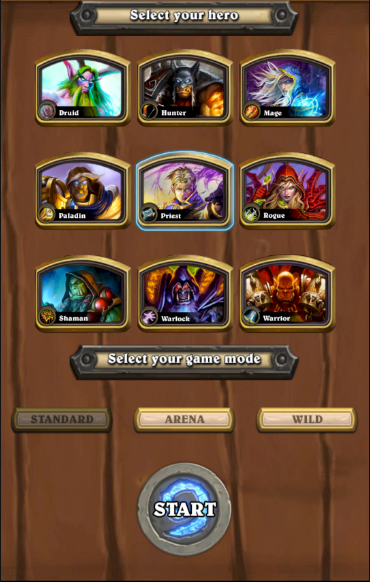
\includegraphics[scale=0.4]{images/screen1}}
        \caption{Sélection du héros adverse}
    \end{minipage} \hfill%
    \begin{minipage}[c]{.46\linewidth}
        \centering
        \fbox{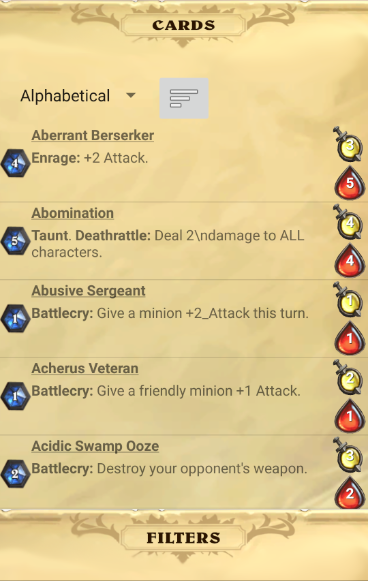
\includegraphics[scale=0.4]{images/screen2}}
        \caption{Liste de cartes}
    \end{minipage}
\end{figure}

L'utilisateur a ensuite la possibilité de consulter la carte pour obtenir toutes les informations dont il a besoin.

\newpage
\section{Compte rendu personnel (Sylvain Ung)}

J'ai déjà eu avant ce projet une première expérience en développement mobile Android : les techniques de programmation sur cette plate-forme ne m'étaient donc pas totalement inconnues, notamment la notion d'activités au sein d'une application. Néanmoins, mes connaissances étaient plutôt superficielles, ce projet m'a donc permis de les approfondir. J'ai particulièrement apprécié la découverte et l'intégration de bibliothèques externes pour répondre à des besoins spécifiques qui ne pouvaient pas être satisfaits par la SDK Android de base, comme la gestion des GIF.
\paragraph{}
Mes principales contributions au développement de l'application concernait surtout la partie interface utilisateur par la production d'éléments graphiques pertinents et la disposition des layouts qui composent les activités. En effet, l'objectif principal est de rendre l'application agréable à utiliser et intuitive.

\newpage
\section{Compte rendu personnel (Roman Delgado)}

\end{document}